\subsection{External Interface Requirements}
\subsubsection{User Interfaces}
The main way the users can interact with the system is via the mobile application for their smartphone, the interface should be user-friendly and in particular easy to read, with large and high contrast text to minimize reading problems in direct sunlight; the second way of connecting to the services provided is to use the web application their personal computer.
In both cases the user interfaces must satisfy the following constrains:
\begin{itemize}
	\item The first page must always ask the user to login or register to service.
	\item After the login, the system redirects the user to his/her home page.
	\item (Web) A toolbar must be present in every page, except login and registration page.
	\item (Mobile) A toolbar must be present in the homepage.
	\item The \emph{Create a meeting} page must provide a guided process to set-up a meeting and clearly show if the created meeting is not reachable in time from the location of a previous appointment.
	\item The \emph{Manage meetings} page must show a list of user's meetings divided by day and hour, and allows the user to select a meeting to obtain further information.
	\item The interface must offer the possibility to choose between a set of different languages.
	\item The user interface must dynamically adapt to the screen size.
	\item The Mobile and Web application must use the same graphical elements.
\end{itemize}
In addition to these constraints, other platform-dependent constraints are provided:
\begin{itemize}
	\item Web Application:\par
		All the pages must submit to W3C standards.
	\item Mobile Application:\par
		All mobile versions must follow the design guidelines provided by the respective platform manufacturer (Android, iOS, Windows \dots).
\end{itemize}
\subsubsection{Hardware Interfaces}
The web application needs any personal computer connected to the internet, while the mobile application must be able to connect to the network in order to exchange information with the server, such as destination and location of the user retrieved via the GPS of the mobile device.\\
Hardware requirements for both are later specified in \autoref{sec:HardwareLimitations}
\clearpage
\subsubsection{Software Interfaces}
\label{sec:SoftwareInterfaces}
Supported browsers for the web application should include Google Chrome, Mozilla Firefox, Opera, Safari, Internet Explorer and Edge, while the mobile application must be available on Android, iOS, Windows Phone and Blackberry OS.\\
The server side of the application requires: 
\begin{itemize}
	\item \href{http://www.oracle.com/technetwork/java/javaee/overview/index.html}{Java EE}, to write the server application that perform the travel computation and the database access.
	\item \href{https://dev.mysql.com/}{MySQL}, to memorize user information and meetings inside a relational database.
\end{itemize}
The client side of the application requires the latest version of the platform SDK.
\subsubsection{Communication Interfaces}
The client communicates to the server via HTTPS protocol using TCP.\\
In addition, the system must be able to use the API of other application in order to retrieves weather and news about road conditions or strike.

\clearpage

\subsection{Functional Requirements}
\subsubsection{Registration}
\paragraph*{Purpose\\}
The main purpose of the \emph{Registration} use case is to provide the user a service which permits the subscription to the system. The user must fill a registration form with his/her personal information and accept the Terms and Conditions of use. After that a confirmation e-mail is sent to the specified e-mail.
\paragraph{Functional Requirements}
\begin{enumerate}[label=R.\arabic*:]
	\item {\label{req:alreadyregistered}}The system must not accept an already registered e-mail.
	\item {\label{req:userinformation}}The user must provide the following information:
	\begin{itemize}
		\item name
		\item surname
		\item e-mail
		\item password
	\end{itemize}
	\item {\label{req:conditionsaccepted}}The system cannot allow the user to proceed in the registration process if he/she does not accept the Terms and Conditions of use.
	\item The system must send an e-mail to the user after he/she submits the form.	
	\item The system must generate a unique link for the registration e-mail.
	\item The user must be able to exit the form any time.
\end{enumerate}

\paragraph*{Use Case\\}
The \emph{Registration} use case is analysed in \autoref{tab:registrationTAB}
\paragraph*{Activity Diagram\\}
The activity diagram of the \emph{Registration} use case in showed in \autoref{fig:registrationac}
\paragraph*{Sequence Diagram\\}
The sequence diagram of the \emph{Registration} use case in showed in \autoref{fig:registrationsq}
\newpage
\begin{longtable}{p{0.25\linewidth}|p{0.75\linewidth}}
	\hline
		\label{tab:registrationTAB}
	\textbf{Name} & \textbf{Registration} \\
	\hline
	\textbf{Actors} & Non registered User \\
	\hline
	\textbf{Entry conditions} & \_ \\
	\hline
	\textbf{Flow of events} & 
	\begin{enumerate}
		\item The user asks to the system to register to its service.
		\item The system shows the appropriate form to fill.
		\item The user fills the form inserting its own information.
		\item The user submits the form.
		\item The system checks if the e-mail is unique.
		\item The system sends to the specified e-mail address a confirmation e-mail with a unique link.
		\item The user must open the e-mail and click on the confirmation link.
		\item The system receives the confirmation, saves the data inside a database and notifies to the user.
	\end{enumerate}\\
	\hline
	\textbf{Exit conditions} & The user is now registered and he/she can login and start to use the service.\\
	\hline
	\textbf{Exceptions} & Exceptions can occur when requirements~\ref{req:alreadyregistered},~\ref{req:userinformation},~\ref{req:conditionsaccepted} are violated, in this case the system reloads the registration form and goes back to step 2. 
	Registration process is also aborted when the user decides to complete it. \\
	\hline
	\caption{\emph{Registration} use case description}
\end{longtable}

\begin{figure}[h]
	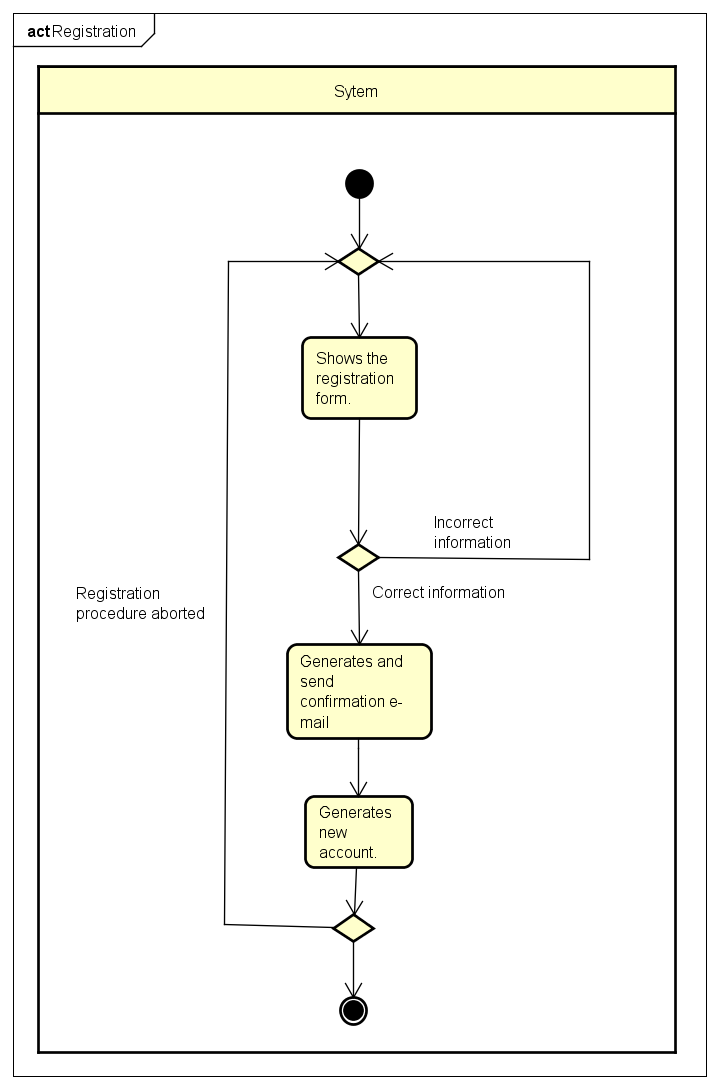
\includegraphics[width=\textwidth, height=\textheight, keepaspectratio=true]{Img/RegistrationAC}
	\caption{\emph{Registration} activity diagram}
	\label{fig:registrationac}
\end{figure}

\begin{sidewaysfigure}
	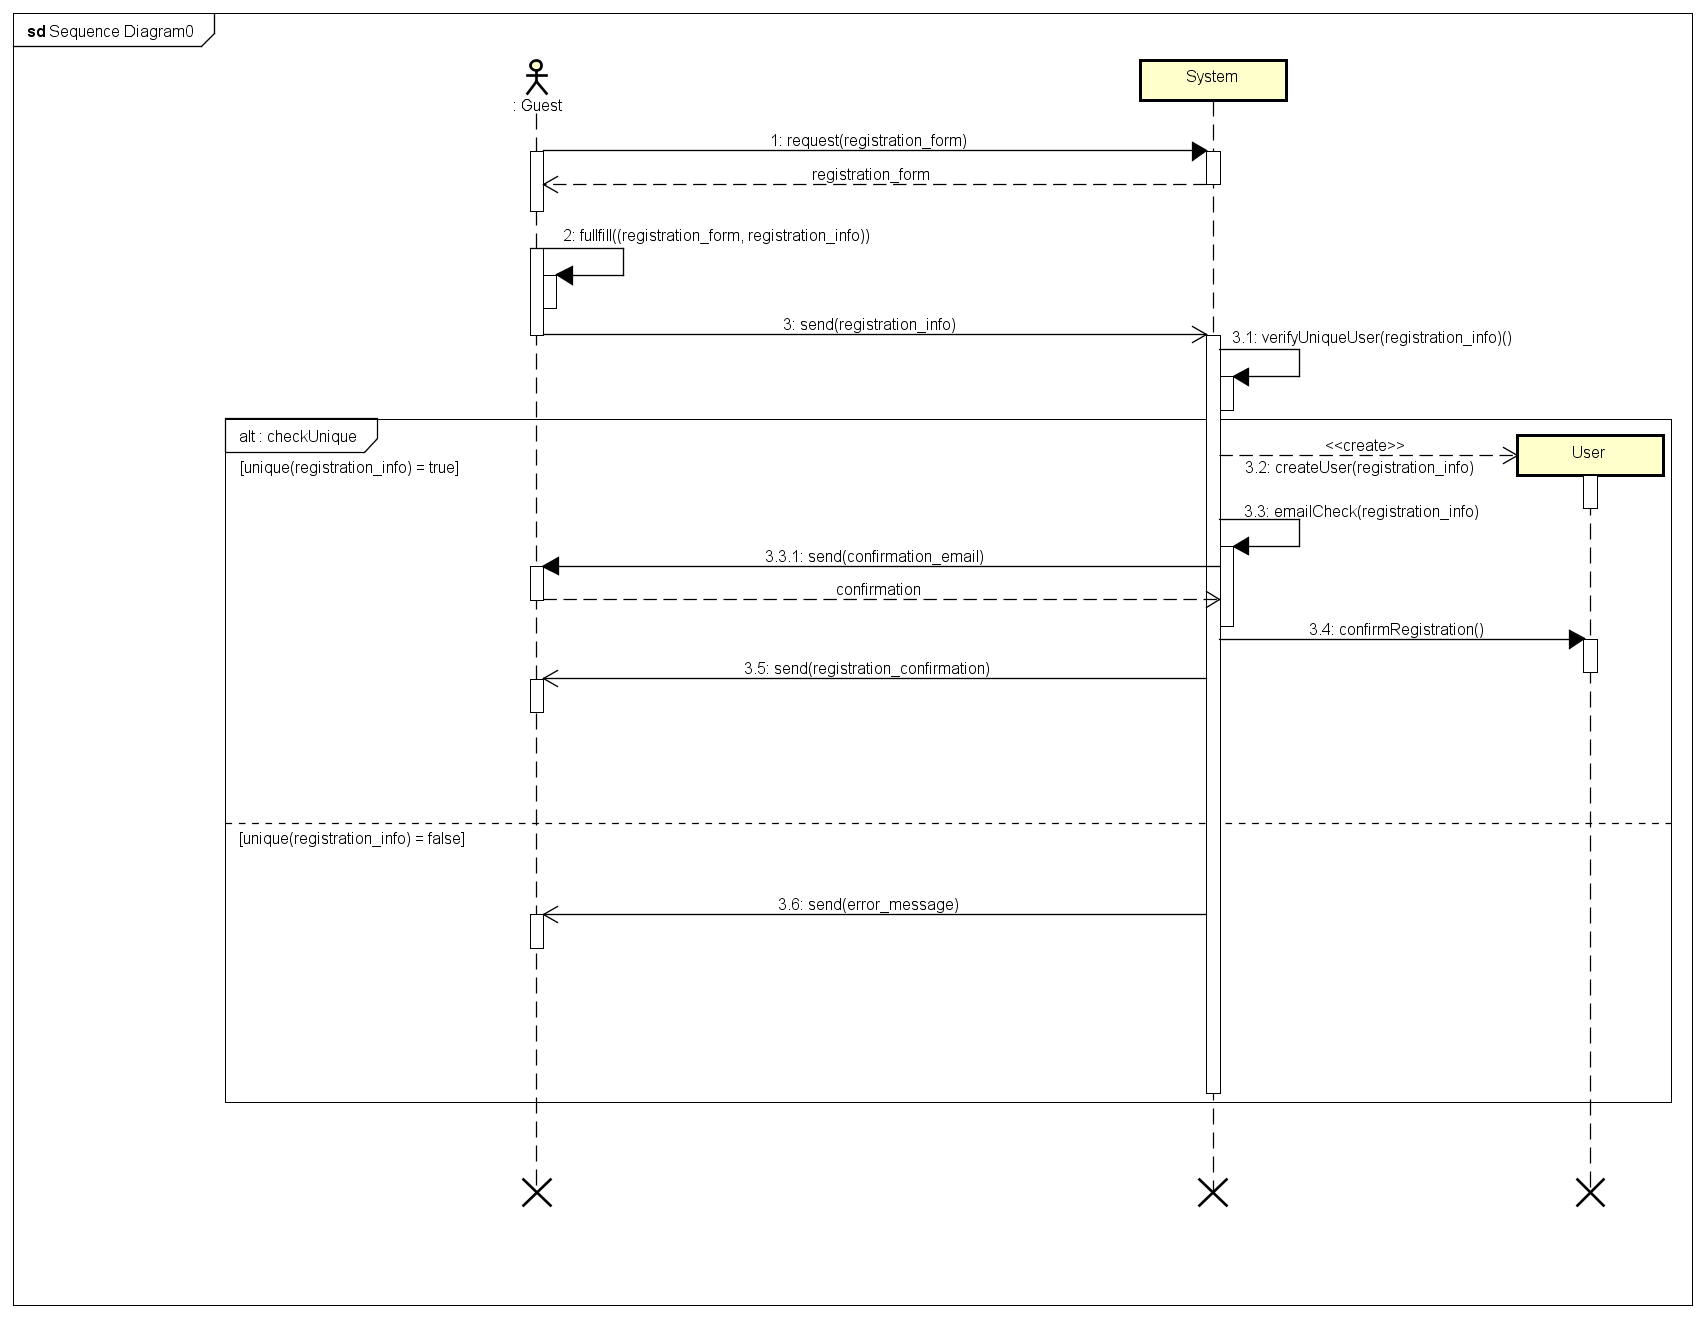
\includegraphics[width=\textheight, height=\textwidth, keepaspectratio=true]{Img/RegistrationSQ}
	\caption{\emph{Registration} sequence diagram}
	\label{fig:registrationsq}
\end{sidewaysfigure}

\clearpage
\subsubsection{Login}
\paragraph*{Purpose\\}
The purpose of \emph{Login} functionality is grant access to \emph{Travlendar+} to any registered user. The system requires an already inserted e-mail and corresponding password in order to access the service.

\paragraph*{Functional Requirements}
\begin{enumerate}[label=R.\arabic*:,resume]
	\item The user must be already registered to the system to perform a successful login.
	\item The system must require the user to insert his/her e-mail and password to perform a login.
	\item The system must check if the password corresponds to a registered e-mail.
	\item The system grants access to its service only to authenticated users.
	\item The user can insert a new password if and only if he/she is a registered user and clicks on "\emph{Forgot my password}".
	\item The password must correspond to the most recent one associated to the user's e-mail.
\end{enumerate}

\paragraph*{Use Case\\}
The \emph{Login} use case is analysed in \autoref{tab:loginTAB}.
\paragraph*{Activity Diagram\\}
The activity diagram of the \emph{Login} use case in showed in \autoref{fig:loginac}.
\paragraph*{Sequence Diagram\\}
The sequence diagram of the \emph{Login} use case in showed in \autoref{fig:loginsq}.

\begin{longtable}{p{0.25\linewidth}|p{0.75\linewidth}}
	\hline
	\label{tab:loginTAB}
	\textbf{Name} & \textbf{Login} \\
	\hline
	\textbf{Actors} & Non registered User \\
	\hline
	\textbf{Entry conditions} & The user is already registered into the system and wants to login. \\
	\hline
	\textbf{Flow of events} & 
	\begin{enumerate}
		\item The user asks to the system to perform a login.
		\item The system shows the \emph{Login} page.
		\item The user inserts his/her e-mail and password and submits.
		\item The system checks if the e-mail corresponds to a registered e-mail.
		\item The system checks if the password is associated to the entered e-mail.
	\end{enumerate}\\
	\hline
	\textbf{Exit conditions} & The user is now logged in.\\
	\hline
	\textbf{Exceptions} & Exceptions occurs when the e-mail has never been registered to the system or when the password does not corresponds to the e-mail.\\
	\hline
	\caption{\emph{Login} use case description}
\end{longtable}

\begin{figure}
	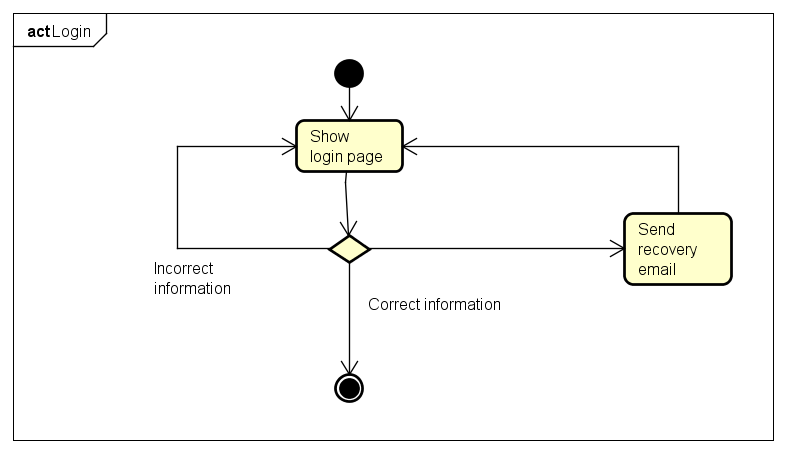
\includegraphics[width=\textwidth, height=\textheight, keepaspectratio=true]{Img/LoginAC}
	\caption{\emph{Login} activity diagram}
	\label{fig:loginac}
\end{figure}

\begin{figure}
	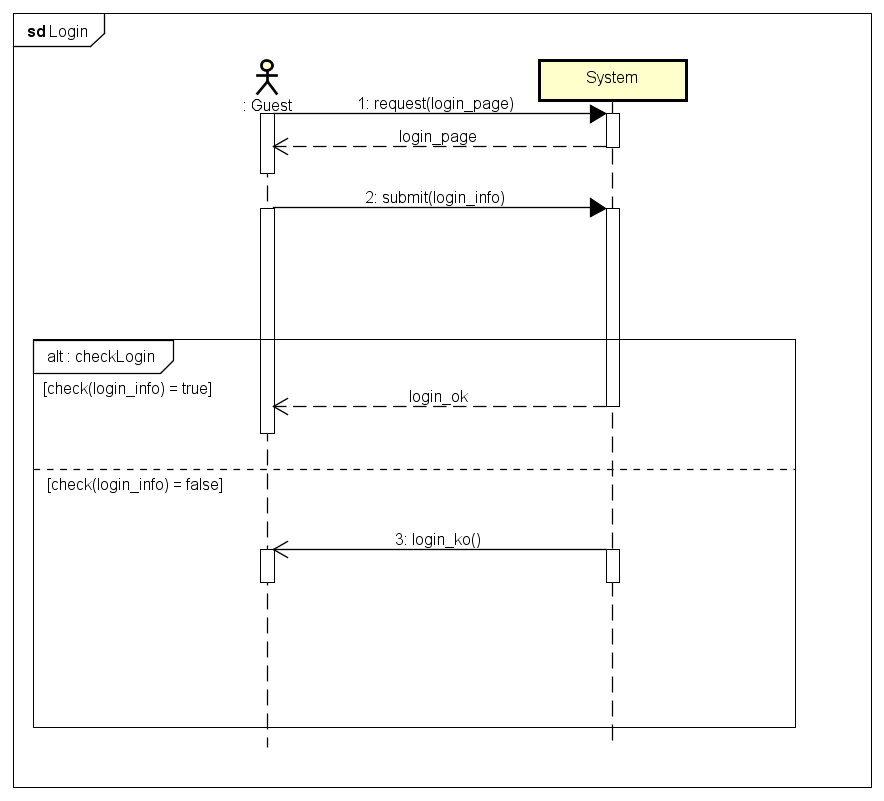
\includegraphics[width=\textwidth, height=\textheight, keepaspectratio=true]{Img/LoginSQ}
	\caption{\emph{Login} sequence diagram}
	\label{fig:loginsq}
\end{figure}

\clearpage
\subsubsection{Specify Means of Travel}
\paragraph*{Purpose\\}
The purpose of this functionality is to allow the user to select an order for his/her favourite means of travel and what vehicles he/she owns, the system will then take this data in consideration once it has to calculate a trip plan by giving precedence to the vehicles higher in the hierarchy.
Both preferred and owned vehicles are optional information, if the user doesn't insert them the system will simply not be influenced when computing travels.

\paragraph*{Functional Requirements}
\begin{enumerate}[label=R.\arabic*:,resume]
	\item The user must be logged in.
	\item A vehicle already selected in an option must not appear again in the list when the user is selecting one.
	\item The user must be able to change the inserted data at any time.
	\item The system must take the preferences into account each time it computes a travel.
\end{enumerate}

\paragraph*{Scenario\\}
Bill loves to move using his bicycle, and wishes to use it each time he can, so he decides to place it as his favourite vehicle by opening the Travlendar + app and after logging in he selects the "Options" icon, then he proceeds to open the "Select favourite vehicles" section and presses the “+” sign to add one, he then chooses "Bicycle" from the list he is presented with.\\
Bill then remembers to also add the Bicycle to his owned vehicles, so the app won't suggest him to use a bike sharing company, to do that he selects the "Owned vehicles" option and just like before he presses the “+” sign and then picks "Bicycle" from the list to add it.

\paragraph*{Use Case\\}
The \emph{Specify Means of Travel} use case is analysed in \autoref{tab:SpecifyMeansofTravelTAB} and in \autoref{fig:SpecifyMeansofTravelUC}
\paragraph*{Activity Diagram\\}
The activity diagram of the \emph{Specify Means of Travel} use case in showed in \autoref{fig:SpecifyMeansofTravelAC}
\paragraph*{Sequence Diagram\\}
The sequence diagram of the \emph{Specify Means of Travel} use case in showed in \autoref{fig:SpecifyMeansofTravelSQ}
\newpage
\begin{longtable}{p{0.25\linewidth}|p{0.75\linewidth}}
	\hline
		\label{tab:SpecifyMeansofTravelTAB}
	\textbf{Name} & \textbf{Specify Means of Travel} \\
	\hline
	\textbf{Actors} & User \\
	\hline
	\textbf{Entry conditions} & The user must be logged in\\
	\hline
	\textbf{Flow of events} & 
	\begin{enumerate}
		\item The user opens the app's options.
		\item The user selects either the option to order the vehicles preferences or the one to add an owned one.
		\item The user selects the “+” sign to add a vehicle.
		\item The system provides a list of vehicles not already selected to the user.
		\item The user chooses a vehicle from the list.
		\item The system stores the choice in the database.
	\end{enumerate}\\
	\hline
	\textbf{Exit conditions} & The user has selected one or more vehicles in his/her preference and/or in the owned section.\\
	\hline
	\textbf{Exceptions} & If the use already selected all possible vehicles the system won’t allow another insertion. \\
	\hline
	\caption{\emph{Specify Means of Travel} use case description}
\end{longtable}

\begin{figure}[h]
	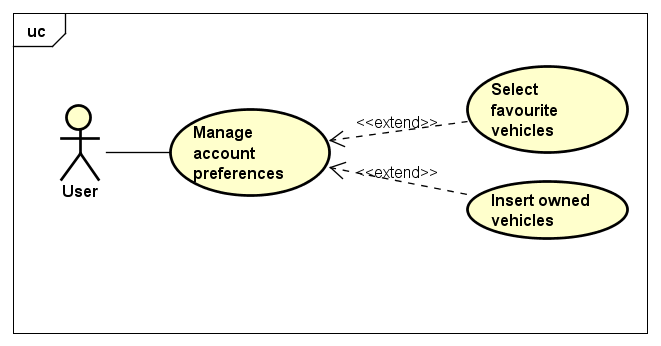
\includegraphics[width=\textwidth]{Img/SpecifyMeansofTravelUC}
	\caption{\emph{Specify Means of Travel} use case}
	\label{fig:SpecifyMeansofTravelUC}
\end{figure}

\begin{figure}[h]
	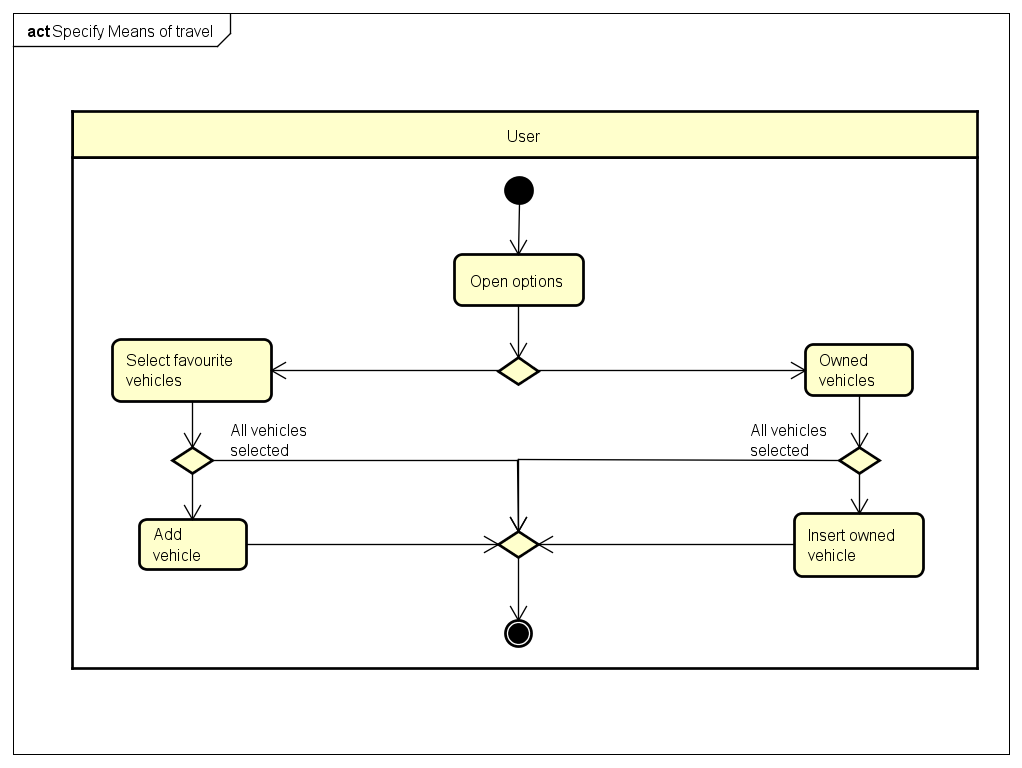
\includegraphics[width=\textheight, height=\textwidth, angle=90, keepaspectratio=true]{Img/SpecifyMeansofTravelAC}
	\caption{\emph{Specify Means of Travel} activity diagram}
	\label{fig:SpecifyMeansofTravelAC}
\end{figure}

\begin{figure}
	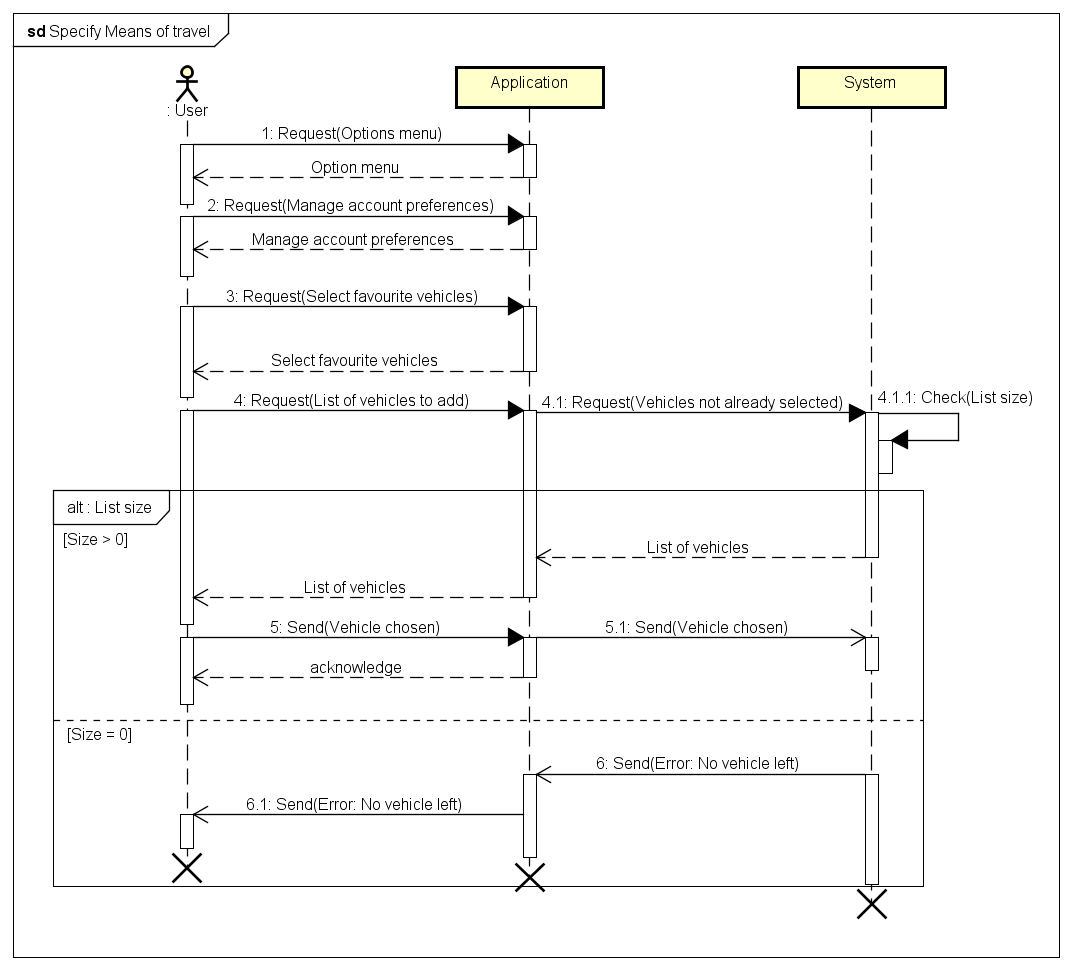
\includegraphics[width=\textheight, height=\textwidth, angle=90, keepaspectratio=true]{Img/SpecifyMeansofTravelSQ}
	\caption{\emph{Specify Means of Travel} sequence diagram}
	\label{fig:SpecifyMeansofTravelSQ}
\end{figure}


\clearpage
\subsubsection{Create Appointment}
\paragraph*{Purpose\\}
This function allows the user to create and register an appointment in the calendar. The user inserts the appointment’s name, the time and location in which occurs and the time and location from where the system must calculate the path. The system then calculates the best path based on the user’s preferences, the weather of appointment day and possible strikes. If the appointment place is not reachable in time the system warns the user.

\paragraph*{Functional Requirements}
\begin{enumerate}[label=R.\arabic*:, resume]
	\item The user must be logged in.
	\item The user must be able to abort the operation any time.
	\item {\label{req:appointmentinformation}}The user must insert:
	\begin{itemize}
		\item Appointment name.
		\item Appointment time and location.
		\item Starting time and location.		
	\end{itemize}
	\item The starting and destination locations must exists.
	\item The appointment time must be after the starting time.
	\item Both the appointment time and the starting time must not be in the past.
	\item If the appointment is not reachable in time a warning must alert the user.
	\item If the appointment duration overlaps with a previous created appointment, a warning must alert the user.
	\item If between the starting time and the appointment time there are one or more appointments, a warning must alert the user.
	\item The user must be able to adjust appointment information after a warning.
	\item The user must be able to ignore the warning if and only if the appointment does not overlaps with others previous created appointments.
	\item The system must calculate the best path every time the appointment information changes.
\end{enumerate}

\paragraph*{Scenario\\}

\paragraph*{Use Case\\}
The \emph{Create Appointment} use case is analysed in \autoref{tab:createappointment} and in \autoref{fig:createappointment}.

\paragraph*{Activity Diagram\\}
The \emph{Create Appointment} activity diagram is showed in \autoref{fig:createappointmentac}.

\paragraph*{Sequence Diagram\\}
The \emph{Create Appointment} sequence diagram is showed in \autoref{fig:createappointmentsq}.

\begin{figure}[h]
	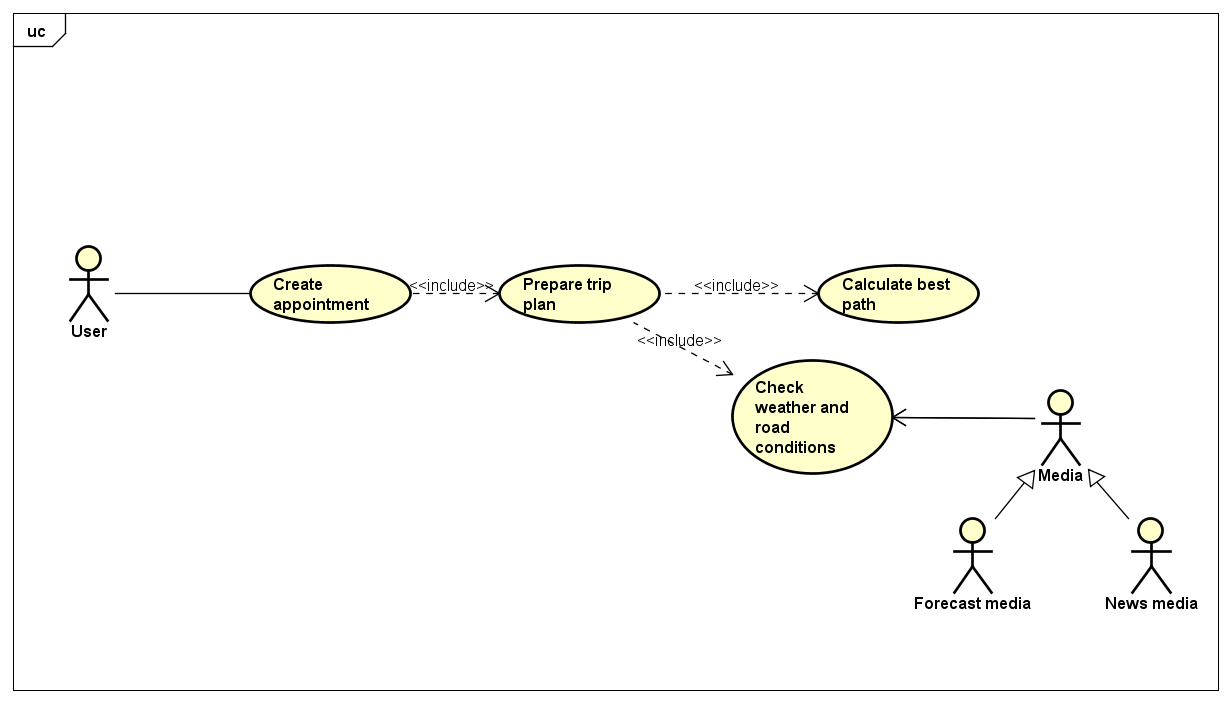
\includegraphics[width=\textwidth, keepaspectratio=true]{Img/CreateAppointmentUC}
	\caption{\emph{Create Appointment} use case}
	\label{fig:createappointment}
\end{figure}

\newpage
\begin{longtable}{p{0.25\linewidth}|p{0.75\linewidth}}
	\hline
	\label{tab:createappointment}
	\textbf{Name} & \textbf{Create appointment} \\
	\hline
	\textbf{Actors} & User \\
	\hline
	\textbf{Entry conditions} & The user must be logged in\\
	\hline
	\textbf{Flow of events} & 
	\begin{enumerate}
		\item The user select "\emph{Create an appointment}.
		\item The user fills the form inserting the data required by the requirement~\ref{req:appointmentinformation}.
		\item The system calculates the best path.
	\end{enumerate}\\
	\hline
	\textbf{Exit conditions} & The system saves the appointment informations.\\
	\hline
	\textbf{Exceptions} & Exceptions can occur when information about time and location of the appointment does not follows the requirements, in this case a warning is generated.
	If the warning is about the non-reachability of the appointment in time the system asks to the user if he/she wants to modify appointment information or to ignore the warning.
	Instead, if the created appointment overlaps with another appointment the system warns the user asking to modify appointment information.
	If the created appointment does not overlaps with other appointments, but is not reachable in time the user can choose to ignore the warning and let the system to create the appointment.
	If the user chooses to abort the operation the appointment will not be saved.
	 \\
	\hline
	\caption{\emph{Create Appointment} use case description}
\end{longtable}

\begin{figure}
	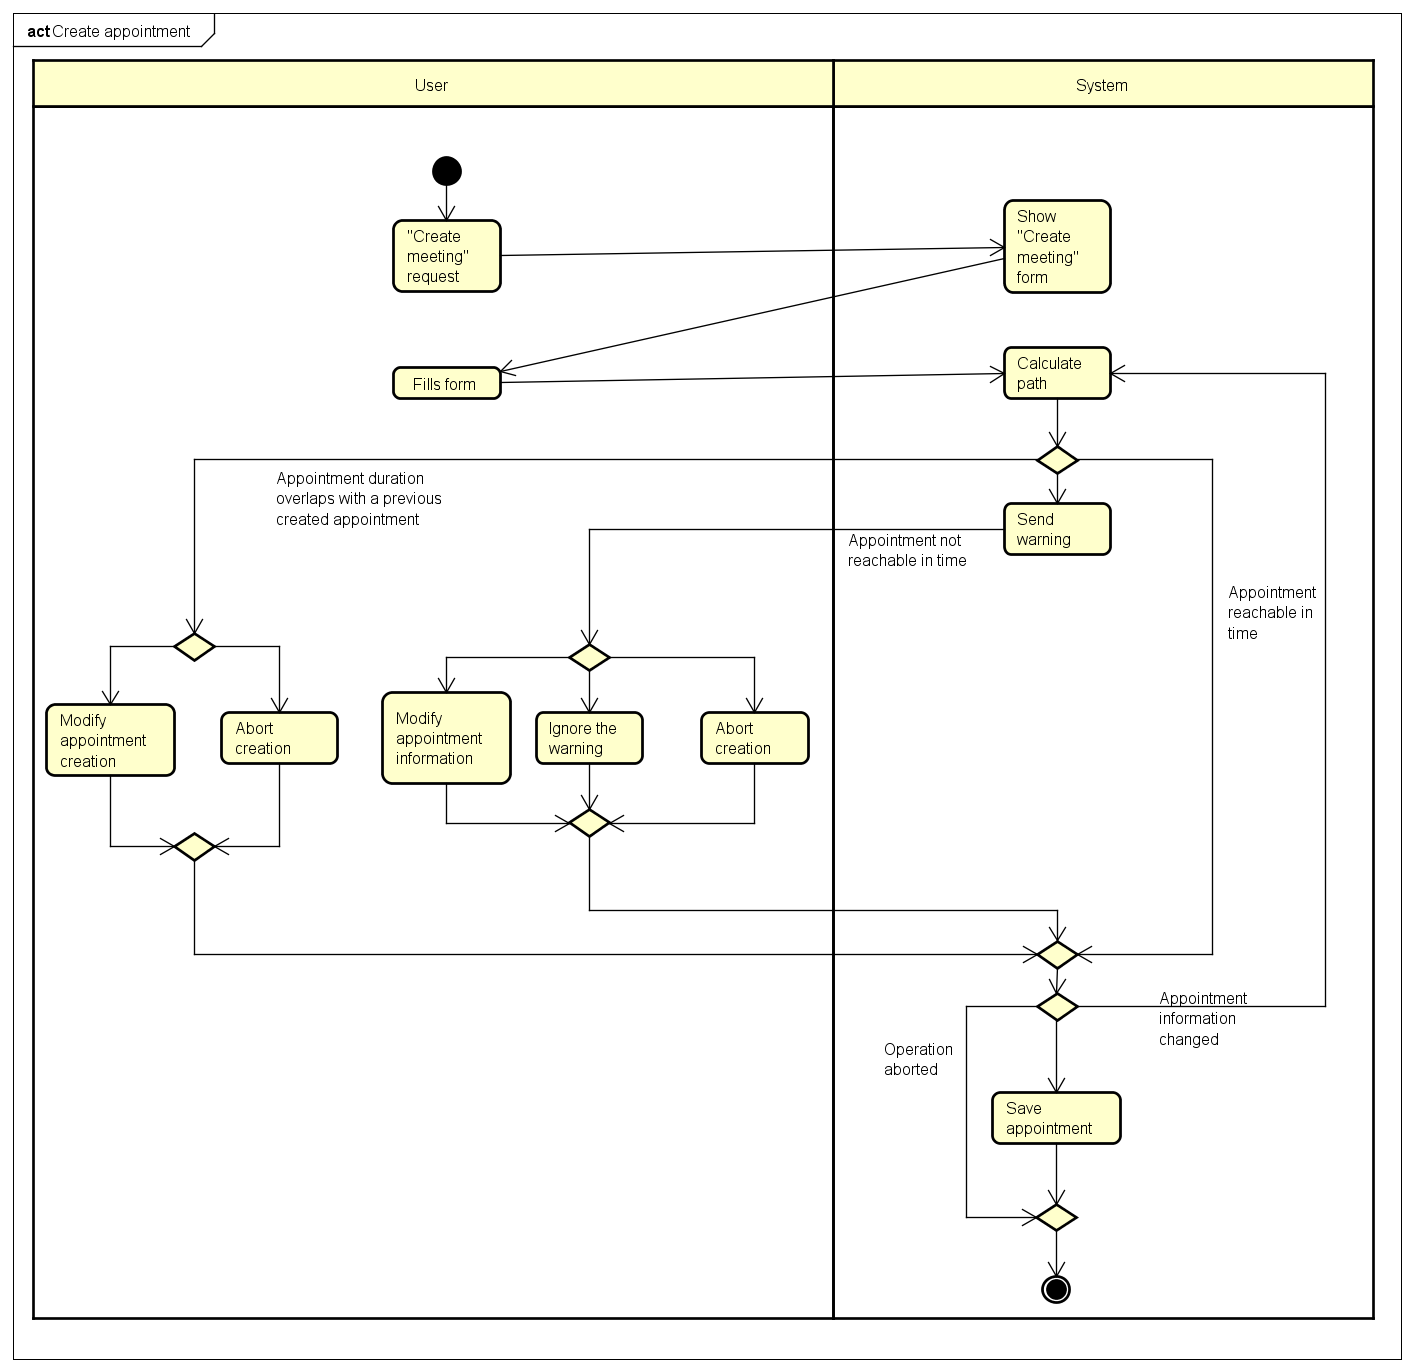
\includegraphics[width=\textwidth, height=\textheight, keepaspectratio=true]{Img/CreateAppointmentAC}
	\caption{\emph{Create Appointment} activity diagram}
	\label{fig:createappointmentac}
\end{figure}

\begin{figure}
	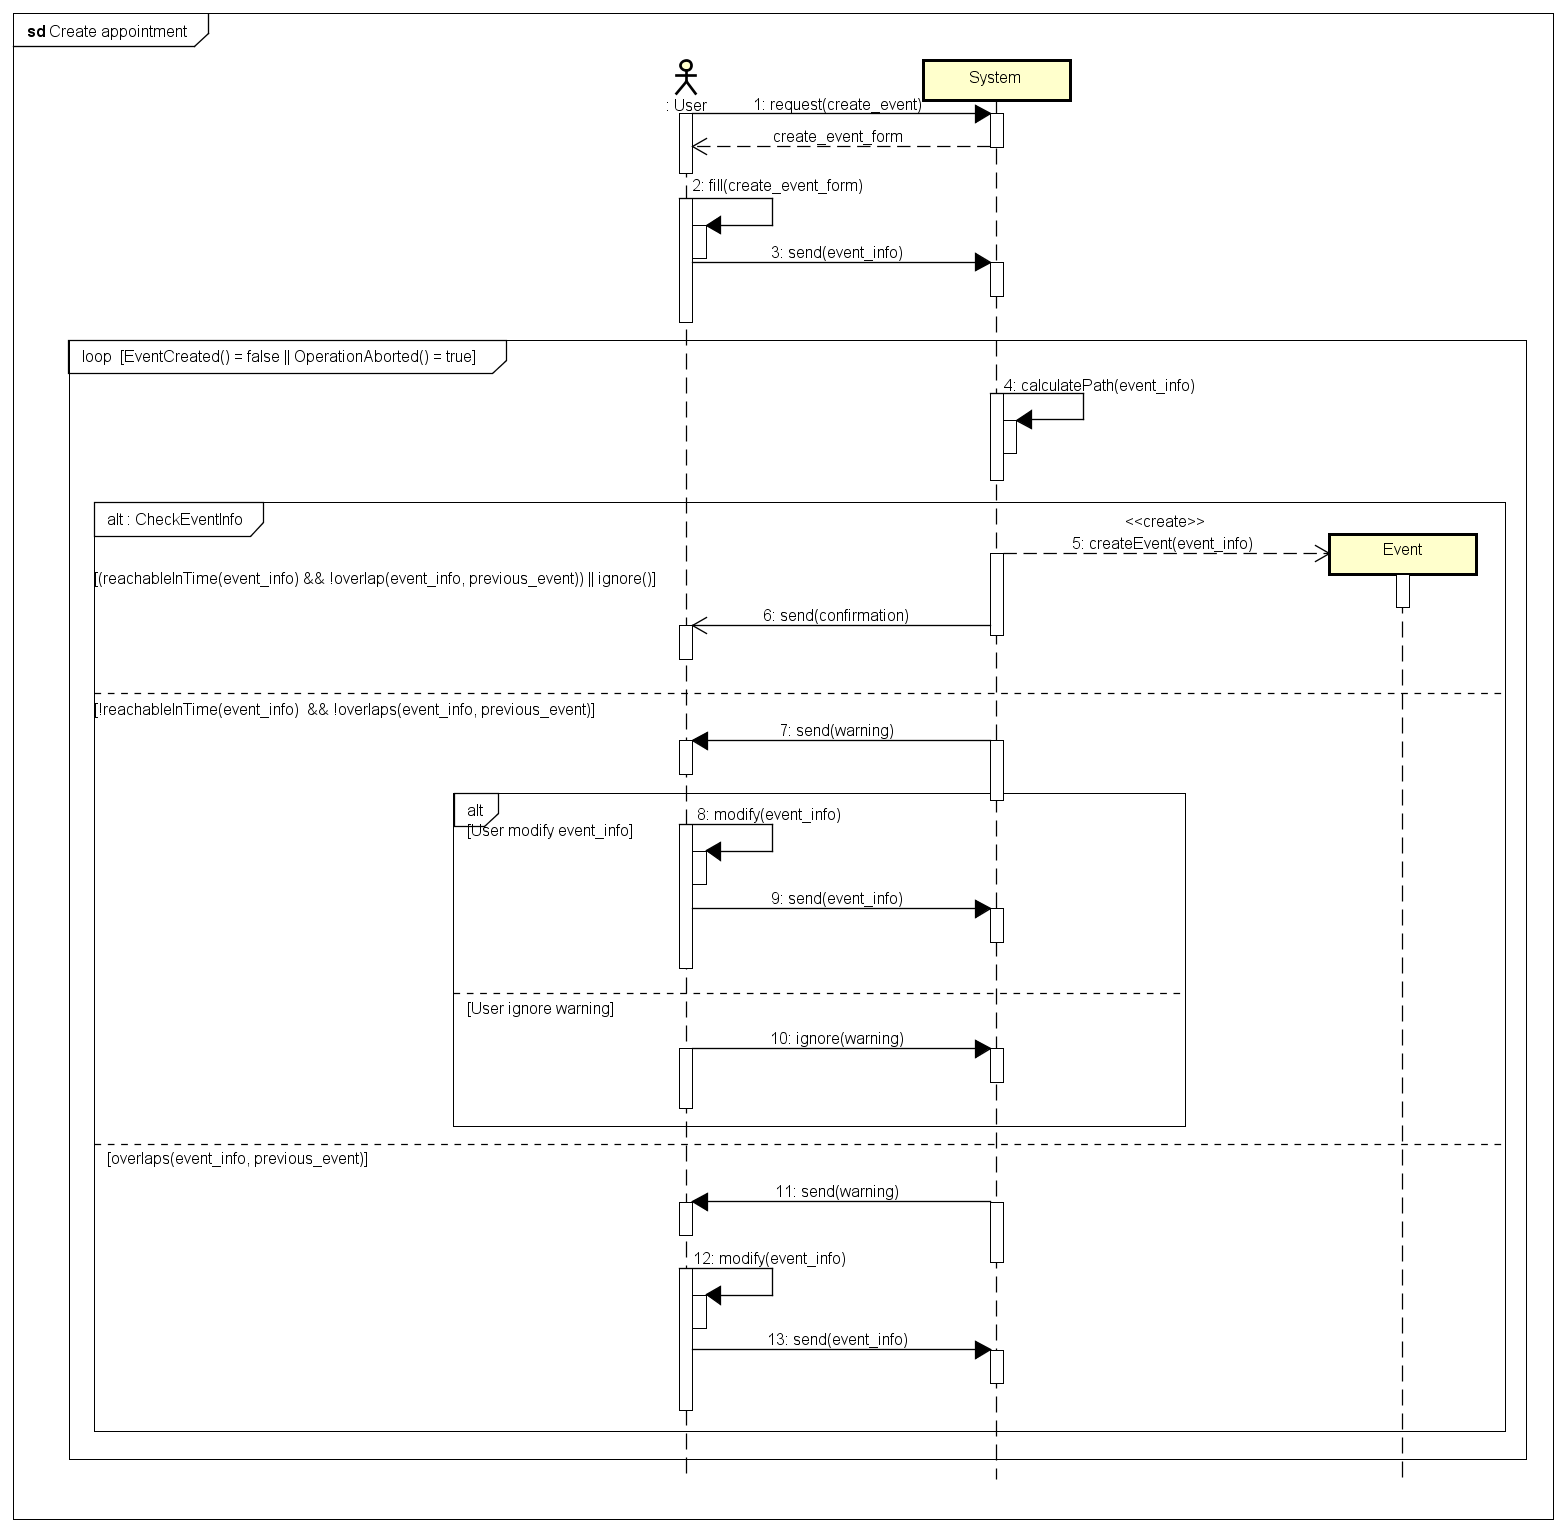
\includegraphics[width=\textwidth, height=\textheight, keepaspectratio=true]{Img/CreateAppointmentSQ}
	\caption{\emph{Create Appointment} sequence diagram}
	\label{fig:createappointmentsq}
\end{figure}

\clearpage
\subsubsection{Change Appointment Information}
\label{ChangeAppointmentInformation}
\paragraph*{Purpose\\}
This function allows the user to select an appointment already registered in the calendar and then change parameters ash he/she wishes, the system will then compute again the trip and store the changes made in the database.
\paragraph*{Functional Requirements}
\begin{enumerate}[label=R.\arabic*:,resume]
	\item The user must be logged in.
	\item The user must have at least one upcoming event saved.
	\item The user must be able to change information as many times as he/she wishes.
	\item Past events cannot be changed.
\end{enumerate}

\paragraph*{Scenario\\}
Anna has taken an appointment with her doctor for next week at 3:00 pm and she already recorded it using Travlendar+, but she remembers that she has to bring her son to football practice before 3:15 pm, she decides then to call her doctor and re-schedules the appointment for 2:00 pm, once the call is finished she opens Travlendar+ and proceeds to open "Manage meetings", and then after selecting the appointment selects "Change meeting details", where she can change the time of the appointment and then saves it.
\paragraph*{Use Case\\}
The \emph{Change Appointment Information} use case is analysed in \autoref{tab:ChangeAppointmentInformationTAB} and in \autoref{fig:ChangeAppointmentInformationUC}
\paragraph*{Activity Diagram\\}
The activity diagram of the \emph{Change Appointment Information} use case in showed in \autoref{fig:ManageAppointmentsAC}
\paragraph*{Sequence Diagram\\}
The sequence diagram of the \emph{Change Appointment Information} use case in showed in \autoref{fig:ChangeAppointmentInformationSQ}
\newpage
\begin{longtable}{p{0.25\linewidth}|p{0.75\linewidth}}
	\hline
		\label{tab:ChangeAppointmentInformationTAB}
	\textbf{Name} & \textbf{Change Appointment Information} \\
	\hline
	\textbf{Actors} & User \\
	\hline
	\textbf{Entry conditions} & The user must be logged in and must have at least one upcoming event.\\
	\hline
	\textbf{Flow of events} & 
	\begin{enumerate}
		\item The user opens the app.
		\item The user selects the "Manage meetings" section.
		\item The user selects the meeting he/she wants to change.
		\item The user selects "Change meeting details".
		\item The user changes the meeting as he/she wishes by providing at least one of the following:
	\begin{enumerate}
	\item Date of the meeting.
	\item Time of the meeting.
	\item Location of the meeting.
	\item Name of the meeting.
	\end{enumerate}
		\item The user saves the changes.
		\item The system updates the meeting in the database and computes again the trip.
	\end{enumerate}\\
	\hline
	\textbf{Exit conditions} & The user changed a meeting.\\
	\hline
	\textbf{Exceptions} & If the meeting has expired and the user tries to change it, the application will avoid it. \\
	\hline
	\caption{\emph{Change Appointment Information} use case description}
\end{longtable}

\begin{figure}[h]
	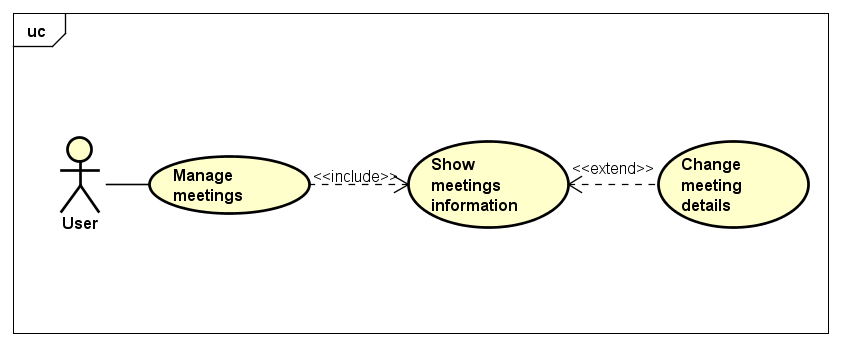
\includegraphics[width=\textwidth]{Img/ChangeAppointmentInformationUC}
	\caption{\emph{Change Appointment Information} use case}
	\label{fig:ChangeAppointmentInformationUC}
\end{figure}

\begin{figure}[h]
\centering
	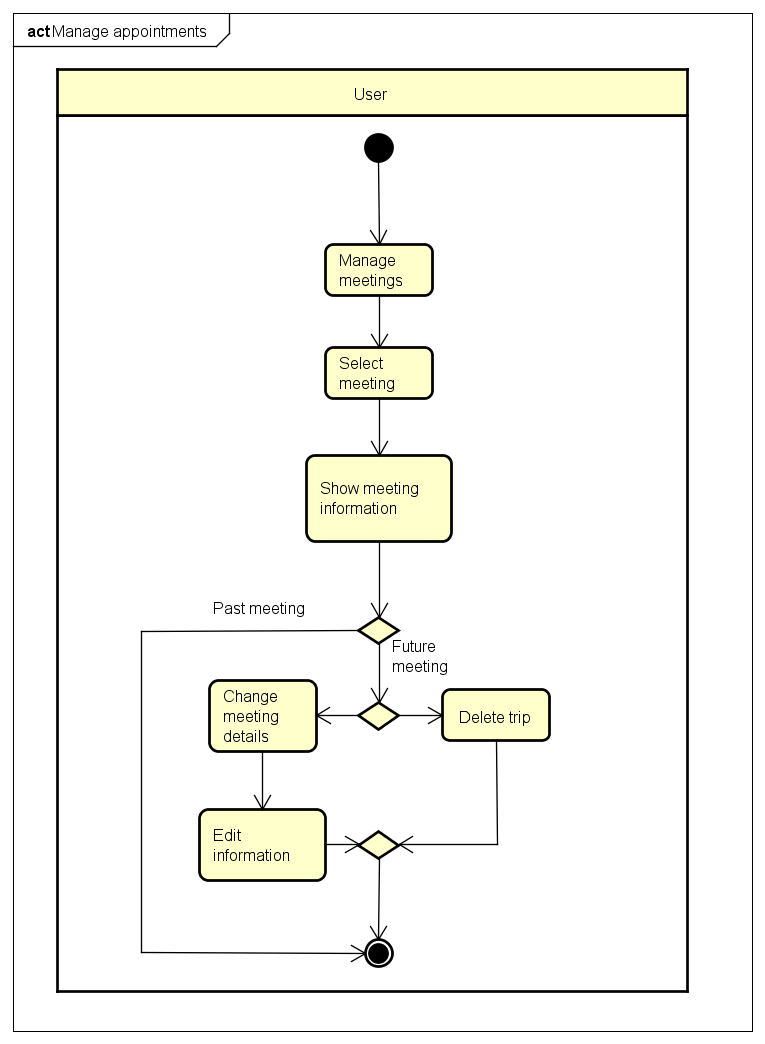
\includegraphics[width=\textheight, height=\textwidth, keepaspectratio=true]{Img/ManageAppointmentsAC}
	\caption{\emph{Change Appointment Information \& Delete Appointment} activity diagram}
	\label{fig:ManageAppointmentsAC}
\end{figure}

\begin{sidewaysfigure}
	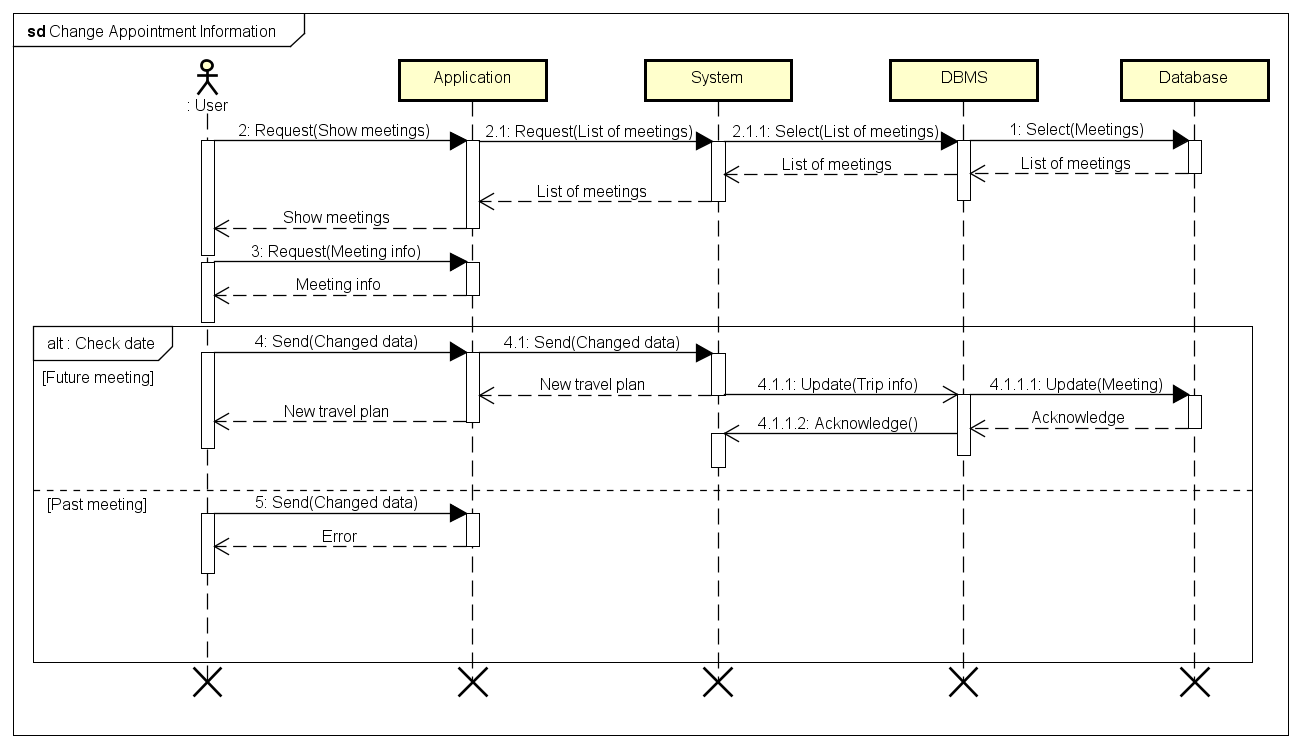
\includegraphics[width=\textheight, height=\textwidth, keepaspectratio=true]{Img/ChangeAppointmentInformationSQ}
	\caption{\emph{Change Appointment Information} sequence diagram}
	\label{fig:ChangeAppointmentInformationSQ}
\end{sidewaysfigure}

\clearpage
\subsubsection{Delete Appointment}
\paragraph*{Purpose\\}
This function allows the user to select an appointment already registered in the calendar and removing it, the system will then notify the DBMS to remove it from the database.
\paragraph*{Functional Requirements}
\begin{enumerate}[label=R.\arabic*:,resume]
	\item The user must be logged in.
	\item The user must have at least one upcoming event saved.
	\item Once a meeting is deleted all data regarding it is lost.
	\item Past events cannot be deleted.
\end{enumerate}

\paragraph*{Scenario\\}
Emily decided with her friends to go out for dinner Saturday and inserted the place and time in a meeting using Travlendar+, but one of the other girls later proposed to have dinner at home, and since Emily has the biggest dining room she invited all the others to her place, since she doesn't need any more a travel planned she deletes the meeting previously created by selecting it in the "Manage meetings" section, she then proceeds to remove it by pressing the "Delete trip" button.
\paragraph*{Use Case\\}
The \emph{Delete Appointment} use case is analysed in \autoref{tab:DeleteAppointmentTAB} and in \autoref{fig:DeleteAppointmentUC}
\paragraph*{Activity Diagram\\}
The activity diagram of the \emph{Delete Appointment} use case in showed in \autoref{fig:ManageAppointmentsAC} alongside \emph{Change Appointment Information} from \autoref{ChangeAppointmentInformation}.
\paragraph*{Sequence Diagram\\}
The sequence diagram of the \emph{Delete Appointment} use case in showed in \autoref{fig:DeleteAppointmentSQ}
\newpage
\begin{longtable}{p{0.25\linewidth}|p{0.75\linewidth}}
	\hline
		\label{tab:DeleteAppointmentTAB}
	\textbf{Name} & \textbf{Delete Appointment} \\
	\hline
	\textbf{Actors} & User \\
	\hline
	\textbf{Entry conditions} & The user must be logged in and must have at least one upcoming event.\\
	\hline
	\textbf{Flow of events} & 
	\begin{enumerate}
		\item The user opens the app.
		\item The user selects the "Manage meetings" section.
		\item The user selects the meeting he/she wants to delete.
		\item The user presses the "Delete trip" button.
		\item The system sends the delete request to the DBMS.
		\item The DBMS deletes the entry selected by the user from the database.
	\end{enumerate}\\
	\hline
	\textbf{Exit conditions} & A meeting was deleted.\\
	\hline
	\textbf{Exceptions} & If the meeting has expired and the user tries to delete it, the application will avoid it. \\
	\hline
	\caption{\emph{Delete Appointment} use case description}
\end{longtable}

\begin{figure}[h]
	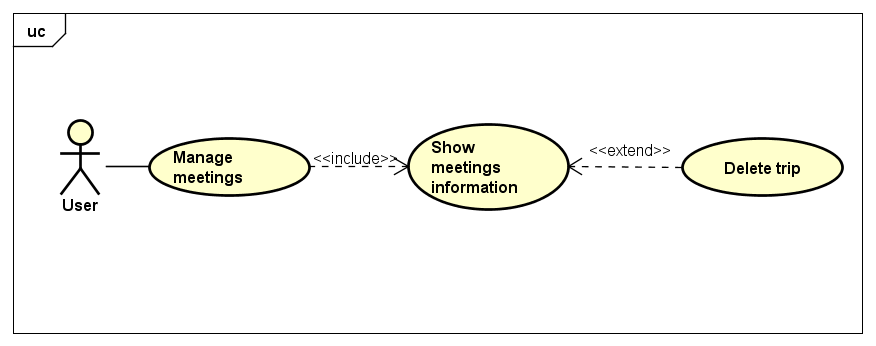
\includegraphics[width=\textwidth]{Img/DeleteAppointmentUC}
	\caption{\emph{Delete Appointment} use case}
	\label{fig:DeleteAppointmentUC}
\end{figure}

\begin{sidewaysfigure}
	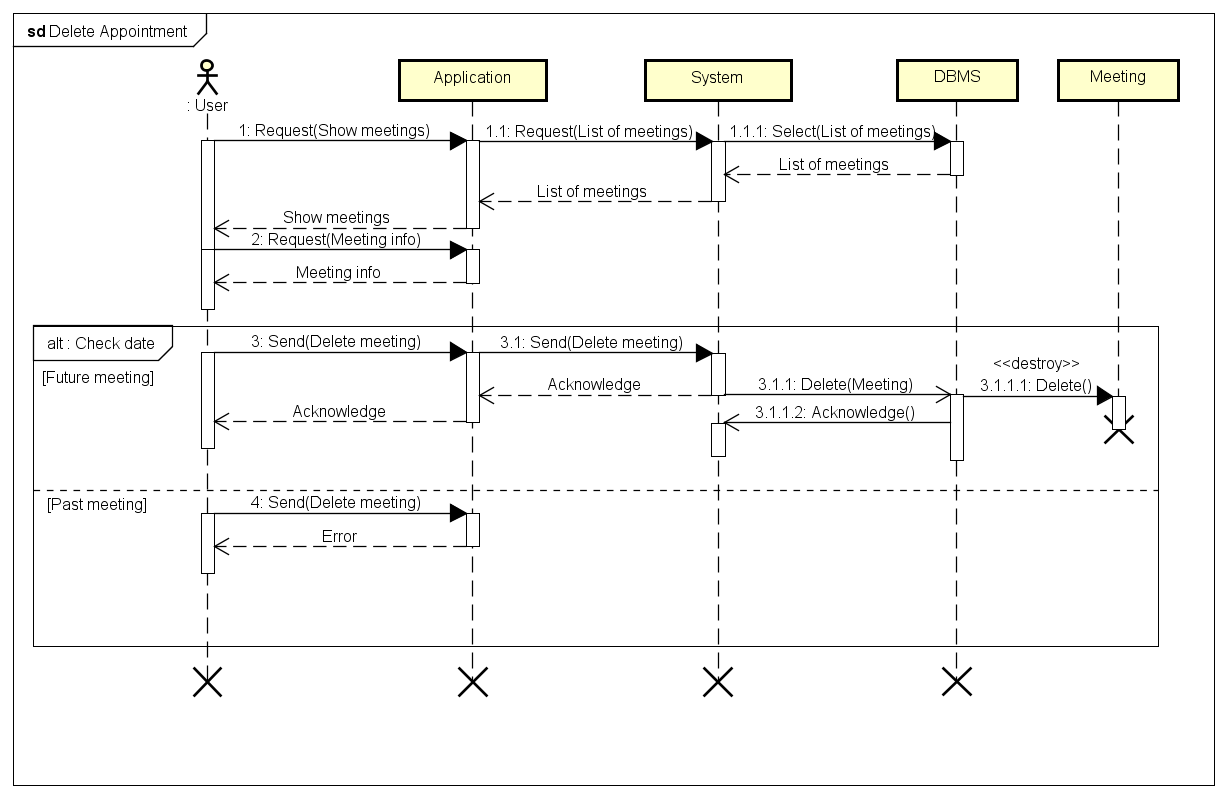
\includegraphics[width=\textheight, height=\textwidth, keepaspectratio=true]{Img/DeleteAppointmentSQ}
	\caption{\emph{Delete Appointment} sequence diagram}
	\label{fig:DeleteAppointmentSQ}
\end{sidewaysfigure}

\clearpage
\subsubsection{Manage Breaks}
\paragraph*{Purpose\\}
The functionality delivered by \emph{Manage Breaks} refers to the possibility of scheduling a flexible time in which the system will reserve a given amount of minutes to any kind of break, with the option of changing or deleting said break in the future.\\
\textbf{Note} that we will focus on the creating aspect, since treating also changing and deleting would offer no additional insight.
\paragraph*{Functional Requirements}
\begin{enumerate}[label=R.\arabic*:,resume]
	\item The user must be logged in.
	\item The user must insert the following parameters:
	\begin{enumerate}
	\item Starting time (From).
	\item Duration of the break.
	\item Days of the week.
	\item End time (To).
	\end{enumerate}
\end{enumerate}
\paragraph*{Scenario\\}
Jimmy has a 3 hours window on Monday between school and soccer practice, from 12:30 am to 15:30 am in which he wants to have lunch and then study the remaining time.\\
He decides to use Travlendar+ to schedule a flexible break, first he opens the app on his smartphone, then after going into "Manage account preferences" he adds a break of 30 minutes in the spare time he has by using the "Create break" option and filling the necessary fields.
\paragraph*{Use Case\\}
The \emph{Create Breaks} use case is analysed in \autoref{tab:CreateBreaksTAB}, in \autoref{fig:ManageBreaksUC} are also represented the "Delete break" and "Change break" functions.
\paragraph*{Activity Diagram\\}
The activity diagram of the \emph{Manage Breaks} use case in showed in \autoref{fig:ManageBreaksAC}
\paragraph*{Sequence Diagram\\}
The sequence diagram of the \emph{Create Breaks} use case in showed in \autoref{fig:CreateBreaksSQ}
\newpage
\begin{longtable}{p{0.25\linewidth}|p{0.75\linewidth}}
	\hline
		\label{tab:CreateBreaksTAB}
	\textbf{Name} & \textbf{Create Breaks} \\
	\hline
	\textbf{Actors} & User \\
	\hline
	\textbf{Entry conditions} & The user must be logged in.\\
	\hline
	\textbf{Flow of events} & 
	\begin{enumerate}
		\item The user opens the app.
		\item The user opens the options menu.
		\item The user enters in "Manage account preferences".
		\item The user selects "Create break".
		\item The user fills the requested fields with the desired information.
		\item The user saves the changes.
		\item The system sends the data to the DBMS.
		\item The DBMS stores the data about the break.
	\end{enumerate}\\
	\hline
	\textbf{Exit conditions} & The user created a break\\
	\hline
	\textbf{Exceptions} & If the user doesn't choose a day of the week the system will act like if every day was selected. \\
	\hline
	\caption{\emph{Create Breaks} use case description}
\end{longtable}

\begin{figure}[h]
	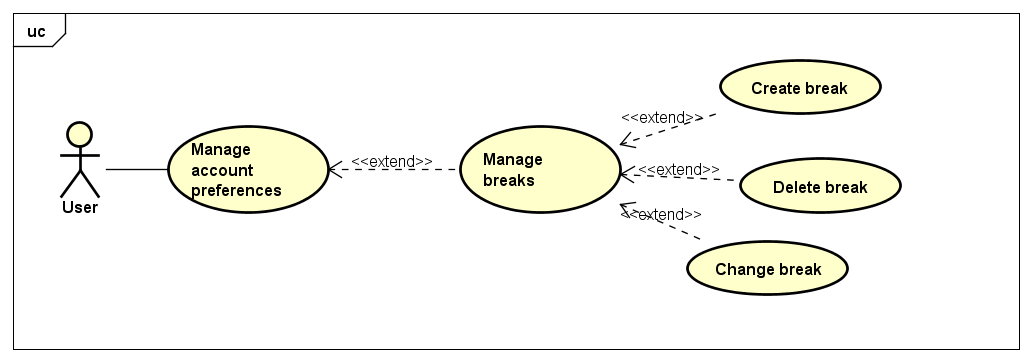
\includegraphics[width=\textwidth]{Img/ManageBreaksUC}
	\caption{\emph{Create Breaks} use case}
	\label{fig:ManageBreaksUC}
\end{figure}

\begin{figure}[h]
\centering
	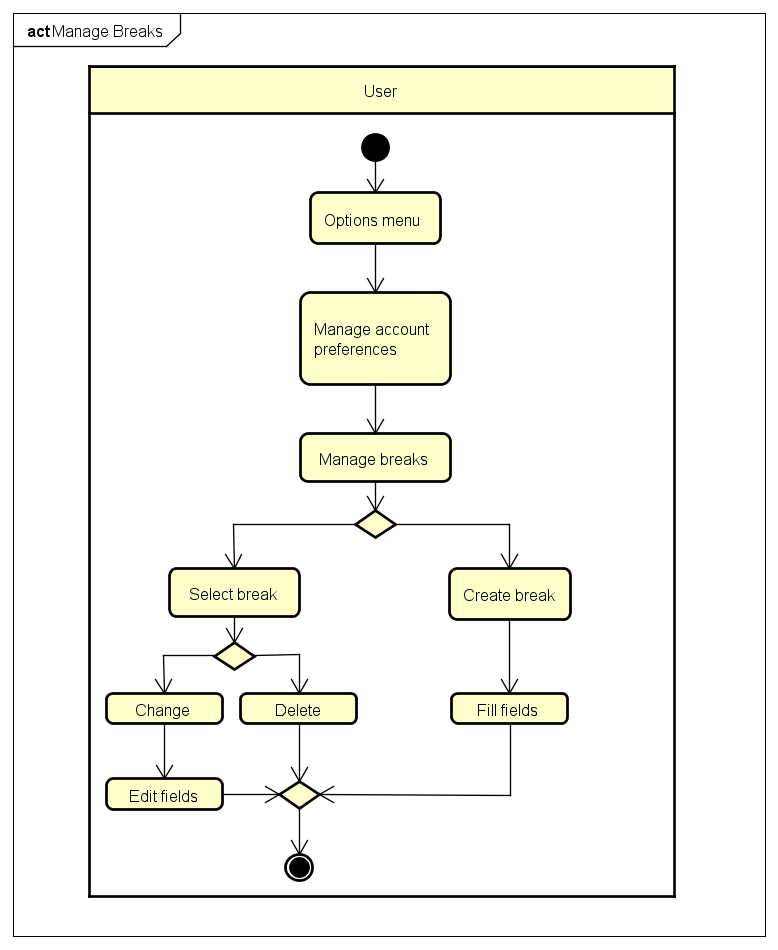
\includegraphics[width=\textheight, height=\textwidth, keepaspectratio=true]{Img/ManageBreaksAC}
	\caption{\emph{Manage Breaks} activity diagram}
	\label{fig:ManageBreaksAC}
\end{figure}

\begin{sidewaysfigure}
	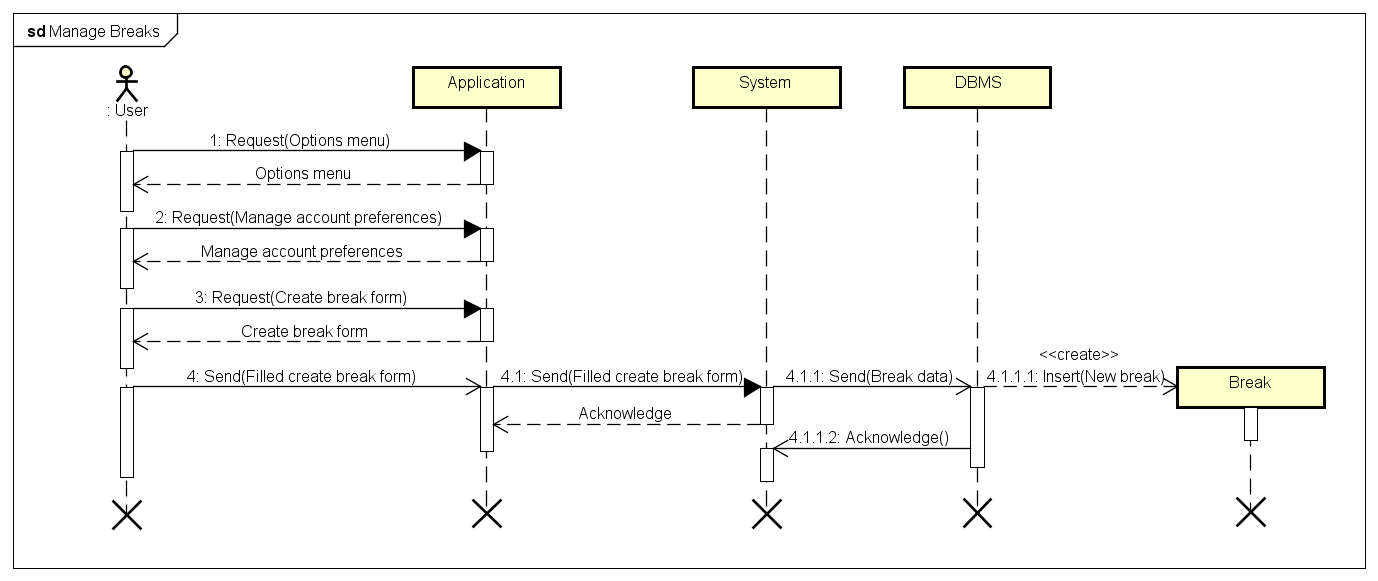
\includegraphics[width=\textheight, height=\textwidth, keepaspectratio=true]{Img/CreateBreaksSQ}
	\caption{\emph{Create Breaks} sequence diagram}
	\label{fig:CreateBreaksSQ}
\end{sidewaysfigure}

\clearpage
\subsubsection{Manage Account}

\paragraph*{Purpose}
The main purpose of this use case is to grant the user the possibility to view his/her personal information, update it or to delete the account.

\paragraph*{Functional Requirements}
\begin{enumerate}[label=R.\arabic*:, resume]
	\item The user must be logged in.
	\item The system must shows all the information inserted during the registration process, except the password.
	\item {\label{req:startmanage}} The system allows the user to update every information except the e-mail used to login.
	\item The user must insert the old password and twice the new password in order to update his/her password.
	\item The system allows to change the password if and only if the old one has been inserted correctly.
	\item {\label{req:endmanage}}The system does not allow the user to update the password if the new one has not been inserted twice.
	\item The system makes every changes permanent as soon as the user confirms the operation.
	\item The user can delete his/her account if and only if he/she inserts the current password.
	\item The system removes from the database the user's personal information if and only if the user deletes his/her account.
\end{enumerate}

\paragraph*{Scenario}

\paragraph*{Use Case}
The use case is analysed in \autoref{fig:manageaccountuc} and in \autoref{tab:viewaccountusecase}, \autoref{tab:modifypersonalinformation} and in \autoref{tab:deleteaccount}.

\begin{figure}[h]
	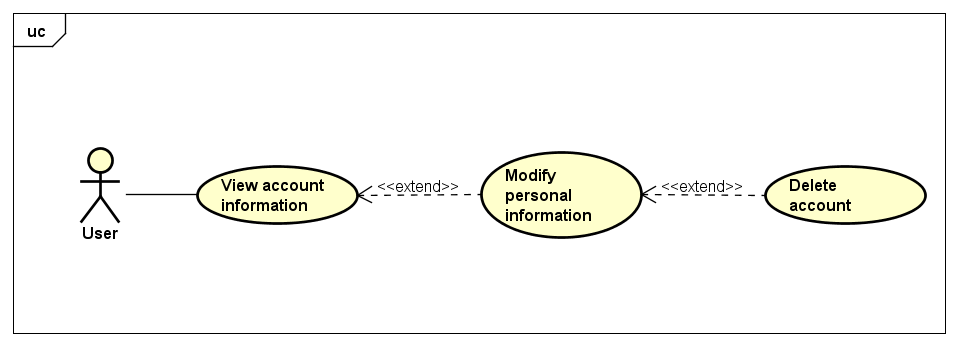
\includegraphics[width=\textwidth, height=\textheight, keepaspectratio=true]{Img/ManageAccountUC}
	\caption{\emph{Manage Account} overall use case}
	\label{fig:manageaccountuc}
\end{figure}

\newpage
\begin{longtable}{p{0.25\linewidth}|p{0.75\linewidth}}
	\hline
	\label{tab:viewaccountusecase}
	\textbf{Name} & \textbf{View account information} \\
	\hline
	\textbf{Actors} & User \\
	\hline
	\textbf{Entry conditions} & The user must be logged in.\\
	\hline
	\textbf{Flow of events} & 
	\begin{enumerate}
		\item The user opens the app.
		\item The user opens the options menu.
		\item The user enters in "Show personal information".
		\item The system shows the user's personal information.
	\end{enumerate}\\
	\hline
	\textbf{Exit conditions} & The system lets the user checks his/her information.\\
	\hline
	\textbf{Exceptions} & \- \\
	\hline
	\caption{\emph{View Account Information} use case description}
\end{longtable}

\begin{longtable}{p{0.25\linewidth}|p{0.75\linewidth}}
	\hline
	\label{tab:modifypersonalinformation}
	\textbf{Name} & \textbf{Modify personal information} \\
	\hline
	\textbf{Actors} & User \\
	\hline
	\textbf{Entry conditions} & The user must be logged in.\\
	\hline
	\textbf{Flow of events} & 
	\begin{enumerate}
		\item The user opens the app.
		\item The user opens the options menu.
		\item The user enters in "\emph{Show personal information}".
		\item The user selects "\emph{Modify my information}".
		\item The user enters the updated information.
		\item The user confirms the changes.
	\end{enumerate}\\
	\hline
	\textbf{Exit conditions} & The system saves the information.\\
	\hline
	\textbf{Exceptions} & If one of the requirements from \ref{req:startmanage} to \ref{req:endmanage} is not satisfied the system ignores the changes and reload the "\emph{Modify my information}" page. \\
	\hline
	\caption{\emph{Modify personal information} use case description}
\end{longtable}

\newpage
\begin{longtable}{p{0.25\linewidth}|p{0.75\linewidth}}
	\hline
	\label{tab:deleteaccount}
	\textbf{Name} & \textbf{Delete account} \\
	\hline
	\textbf{Actors} & User \\
	\hline
	\textbf{Entry conditions} & The user must be logged in.\\
	\hline
	\textbf{Flow of events} & 
	\begin{enumerate}
		\item The user opens the app.
		\item The user opens the options menu.
		\item The user enters in "\emph{Show personal information}".
		\item The user selects "\emph{Modify my information}".
		\item The user selects "\emph{Delete my account}".
		\item The user inserts his/her password.
		\item The user confirms the operation.
	\end{enumerate}\\
	\hline
	\textbf{Exit conditions} & The system deletes the user's account and the user is not registered anymore.\\
	\hline
	\textbf{Exceptions} & If the user enters the wrong password the system prevents the account cancellation. \\
	\hline
	\caption{\emph{Delete account} use case description}
\end{longtable}


%Add Use cases----------------------------------------------------
\clearpage
\subsection{Performance Requirements}
Without taking into consideration the speed of the internet connection, in order to guarantee an acceptable user experience the following  requirements must be satisfied:
\begin{itemize}
\item Navigation between pages of the system must happen in 0.5s or less.
\item The  best travel plan must be computed in 5s or less.
\item No limit of registered users in the database.
\item No limit of schedulable appointments.
\item At least 1000 users must be able to use the service at the same time. 
\end{itemize}
\newpage
\subsection{Design Constraints}
\subsubsection{Standards Compliance}
The web application must comply with the standards dictated by W3C, while the mobile application must follow the Oracle guidelines for Java programming.
\subsubsection{Hardware Limitations}
\label{sec:HardwareLimitations}
Minimum system requirements for the two applications:
\begin{itemize}
\item Web application
\begin{itemize}
\item 512Mb of RAM.
\item 2Mb/s internet connections.
\item 800X600 screen resolution.
\end{itemize}
\item Mobile application
\begin{itemize}
\item 1Gb of RAM.
\item 3G UMTS internet connections.
\item 100Mb of free space.
\end{itemize}
\end{itemize}
The system should also be able to process operations in parallel.
\clearpage
\subsection{Software System Attributes}
\subsubsection{Reliability}
Each trip plan computed given the preferences expressed by the user and the weather forecast and strikes must not differ more than 5\% from the optimal travel distance or ETA.
\subsubsection{Availability}
The system to be must guarantee an availability of no less than 98\%.
\subsubsection{Safety and Privacy Constraints}
The user oversees his/her own security while travelling and must grant access to the current location, information about former trips and personal data are stored but only the user itself has access to them.
\subsubsection{Maintainability}
The system must be developed in such a way that future implementation of new features and changes to existing ones can be done seamlessly, in other words the system has to be modular and scalable.
\subsubsection{Portability}
As already mentioned in \autoref{sec:SoftwareInterfaces} the software must be available on different configurations, it must be as environment independent as possible, meaning that it has to work on different platforms with the minimum amount of changes to the software itself.


